\documentclass[11pt]{article}
\usepackage[margin=18mm,headheight=22pt]{geometry}
\usepackage{amsmath}
\usepackage{fontspec}
\usepackage{unicode-math}
\setmainfont{NewCM10}[Extension=.otf,UprightFont=*-Book,BoldFont=*-Bold,ItalicFont=*-BookItalic,BoldItalicFont=*-BoldItalic]
\setsansfont{NewCMSans10}[Extension=.otf,UprightFont=*-Book,BoldFont=*-Bold,ItalicFont=*-BookOblique,BoldItalicFont=*-BoldOblique]
\setmathfont{NewCMMath-Book.otf}
\usepackage{xcolor}
\definecolor{FAUblue}{HTML}{04316A}
\definecolor{Paperblue}{HTML}{EEF2F7}
\definecolor{EEIgold}{HTML}{CC9C42}
\usepackage{etoolbox,enumitem,booktabs,tabularx,array,needspace,microtype}
\usepackage[most]{tcolorbox}
\usepackage{titlesec,fancyhdr}
\usepackage[hidelinks]{hyperref}
\usepackage{draftwatermark}
\SetWatermarkText{Made by Thanate Amornjiraporn (Focus)}
\SetWatermarkColor{black!7}\SetWatermarkFontSize{30pt}\SetWatermarkAngle{45}
\setlength{\parindent}{0pt}
\setlength{\parskip}{5pt}
\setlist{itemsep=2pt,topsep=3pt,leftmargin=1.6em,beginpenalty=10000,endpenalty=10000}
\raggedbottom
\clubpenalty=10000 \widowpenalty=10000 \displaywidowpenalty=10000 \interlinepenalty=10000
\setcounter{secnumdepth}{0}
\setcounter{tocdepth}{1}
\pagestyle{fancy}\fancyhf{}
\fancyhead[L]{\small\sffamily\color{FAUblue} From Fundamentals to AI Apocalypse · EEI · Exercise 4}
\fancyhead[R]{\small\sffamily Exercise 4: Worked solutions}
\fancyfoot[C]{\small\thepage}
\titleformat{\section}{\Large\bfseries\sffamily\color{FAUblue}}{}{0pt}{}
\titleformat{\subsection}{\large\bfseries\sffamily\color{FAUblue}}{}{0pt}{}
\titlespacing*{\section}{0pt}{16pt}{6pt}
\preto\section{\Needspace{8\baselineskip}}
\preto\subsection{\Needspace{6\baselineskip}}
\newtcolorbox{equationcard}[1]{colback=Paperblue,colframe=Paperblue,boxrule=0pt,arc=0pt,left=10pt,right=10pt,top=6pt,bottom=6pt,title={#1},fonttitle=\small\bfseries\sffamily,coltitle=FAUblue,before skip=8pt,after skip=8pt}
\newtcolorbox{workedbox}[1]{colback=white,colframe=EEIgold,boxrule=0pt,leftrule=3pt,arc=0pt,left=10pt,top=4pt,bottom=4pt,title={#1},fonttitle=\small\bfseries\sffamily,coltitle=FAUblue,attach title to upper={\par},before skip=8pt,after skip=8pt}
\newtcolorbox{recallbox}[1]{colback=white,colframe=FAUblue,boxrule=0pt,leftrule=3pt,arc=0pt,left=10pt,top=4pt,bottom=4pt,title={#1},fonttitle=\small\bfseries\sffamily,coltitle=FAUblue,attach title to upper={\par},before skip=8pt,after skip=8pt}
\usepackage{environ}
\newsavebox\measurebox
% Typeset the section once invisibly to measure it; start a new page if it will not fit in what is left.
\makeatletter
\newif\ifkeep@measuring
\NewEnviron{keepsection}{%
  \ifkeep@measuring \BODY \else
    \edef\keep@sec{\the\value{section}}\edef\keep@sub{\the\value{subsection}}%
    \setbox\measurebox\vbox{\hsize\linewidth\keep@measuringtrue\def\Needspace##1{}\BODY}%
    \setcounter{section}{\keep@sec}\setcounter{subsection}{\keep@sub}%
    \dimen2=\ht\measurebox \advance\dimen2\dp\measurebox
    \dimen@=\textheight
    \ifdim\pagegoal<\maxdimen
      \dimen@=\pagegoal \advance\dimen@-\pagetotal
      \ifdim\dimen2>\dimen@ \clearpage \dimen@=\textheight \fi
    \fi
    % if it fits, nothing inside may force an early break
    \ifdim\dimen2>\dimen@ \BODY \else \begingroup\def\Needspace##1{}\BODY\endgroup \fi
  \fi}
\makeatother
\newtcolorbox{notebox}{colback=Paperblue,colframe=Paperblue,boxrule=0pt,arc=0pt,left=8pt,right=8pt,top=4pt,bottom=4pt,before skip=6pt,after skip=6pt}
\newtcolorbox{plainbox}{colback=white,colframe=FAUblue,boxrule=0pt,leftrule=3pt,arc=0pt,left=10pt,right=8pt,top=4pt,bottom=4pt,before skip=6pt,after skip=8pt}
\usetikzlibrary{arrows.meta}
\title{\sffamily\bfseries\color{FAUblue}Exercise 4: Worked solutions}
\author{Electrical Engineering I \ensuremath{\cdot} Module 92315 \ensuremath{\cdot} Exercise 4\\[2pt]\small From Fundamentals to AI Apocalypse · personal study guide}
\date{}
\begin{document}
\maketitle
\begingroup\footnotesize\setlength{\parskip}{0pt}\tableofcontents\endgroup
\clearpage

\Needspace{9\baselineskip}
{\large Try each part before opening the answer. We apply the interface conditions to the measured field, then use cylindrical Gauss surfaces and voltage integration for the layered coaxial geometry.}


\begin{keepsection}
\Needspace{9\baselineskip}
\section{Task 9: Field at a flat dielectric boundary}

\Needspace{6\baselineskip}
An infinite line charge of density \textit{λ}\textsubscript{0} lies along the z-axis. The lower half-space y \ensuremath{<} h is air with permittivity \textit{ε}\textsubscript{0}, and the upper half-space y \ensuremath{\geq} h has permittivity \textit{ε}\textsubscript{1}. In the air, measurements give the field below.

\Needspace{5\baselineskip}
\begin{equation*}{E}_{0}(\mathrm{x},\mathrm{y})\, =\, \dfrac{{λ}_{0}}{π({ε}_{0}\, +\, {ε}_{1})(\mathrm{x}^{2}\, +\, \mathrm{y}^{2})}\, \left[\mathrm{x}{e}_{\mathrm{x}}\, +\, \dfrac{{ε}_{1}}{{ε}_{0}}\mathrm{y}{e}_{\mathrm{y}}\right]\end{equation*}

\Needspace{9\baselineskip}
\textbf{Connected topic:} Material boundary conditions (§1.11) keep tangential E continuous and normal D continuous when no free surface charge is present.

\Needspace{14\baselineskip}
\begin{center}
\begin{minipage}[t]{0.950\linewidth}\centering
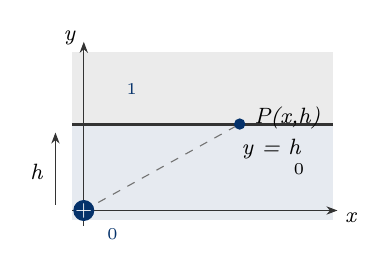
\begin{tikzpicture}[line join=round]
\fill[black!8] (0.756,-0.450) rectangle (4.068,-1.368);
\fill[FAUblue!10] (0.756,-1.368) rectangle (4.068,-2.592);
\draw[black!80,line width=1.1pt] (0.756,-1.368) -- (4.068,-1.368);
\draw[-{Stealth[length=4pt]},black!80] (0.900,-2.664) -- (0.900,-0.324);
\draw[-{Stealth[length=4pt]},black!80] (0.756,-2.466) -- (4.122,-2.466);
\draw[black!55,dashed] (0.900,-2.466) -- (2.880,-1.368);
\filldraw[draw=FAUblue,fill=FAUblue] (0.900,-2.466) circle (0.126);
\node[text=white,font=\footnotesize\bfseries] at (0.900,-2.466) {$+$};
\fill[FAUblue] (2.880,-1.368) circle (0.072);
\draw[-{Stealth[length=4pt]},black!80] (0.540,-2.394) -- (0.540,-1.476);
\node[anchor=west,inner sep=1pt,font=\footnotesize] at (4.176,-2.556) {\textit{x}};
\node[anchor=east,inner sep=1pt,font=\footnotesize] at (0.846,-0.270) {\textit{y}};
\node[text=FAUblue,inner sep=1pt,font=\footnotesize] at (1.476,-0.918) {ε\textsubscript{1}};
\node[,inner sep=1pt,font=\footnotesize] at (3.600,-1.944) {ε\textsubscript{0}};
\node[anchor=west,text=FAUblue,inner sep=1pt,font=\footnotesize] at (1.080,-2.772) {λ\textsubscript{0}};
\node[anchor=east,inner sep=1pt,font=\footnotesize] at (0.432,-1.980) {\textit{h}};
\node[anchor=west,inner sep=1pt,font=\footnotesize] at (3.024,-1.296) {\textit{P(x,h)}};
\node[anchor=west,inner sep=1pt,font=\footnotesize] at (2.862,-1.692) {\textit{y = h}};
\end{tikzpicture}\par\smallskip{\small\raggedright \textbf{Resolve the measured field into interface-parallel and interface-normal parts.} The x-component stays continuous; the y-component changes with permittivity.\par}\end{minipage}
\end{center}

\begin{keepsection}
\Needspace{7\baselineskip}
\subsection{9: Electric field in the dielectric at y = h}

\Needspace{4\baselineskip}
Try first: evaluate the measured air field at the interface, then apply the tangential-E and normal-D boundary conditions component by component.

\nopagebreak[4]{\small\itshape Answers: see “Task 9: Field at a flat dielectric boundary” under Answers at the end.}
\end{keepsection}
\end{keepsection}

\begin{keepsection}
\Needspace{12\baselineskip}
\section{Task 10: Two-dielectric coaxial capacitor}

\Needspace{9\baselineskip}
Two infinitely long concentric metal cylinders share the z-axis. The inner metal’s outer radius is \textit{a}\textsubscript{0}; the outer metal’s inner radius is \textit{a}\textsubscript{2} \ensuremath{>} \textit{a}\textsubscript{0}. Between them, permittivity is \textit{ε}\textsubscript{1} for \textit{a}\textsubscript{0} \ensuremath{<} ρ \ensuremath{<} \textit{a}\textsubscript{1} and \textit{ε}\textsubscript{2} for \textit{a}\textsubscript{1} \ensuremath{<} ρ \ensuremath{<} \textit{a}\textsubscript{2}. The conductor walls each have thickness \textit{d}; outside the conductors is material \textit{ε}\textsubscript{0}. The only charges are σ\textsubscript{0} at the inner conductor’s outer surface and σ\textsubscript{2} at the outer conductor’s inner surface.

\Needspace{9\baselineskip}
\textbf{Connected topics:} Gauss’s law (§1.10) finds the radial flux; capacitance (§1.13) follows from charge per length divided by voltage.

\Needspace{14\baselineskip}
\begin{center}
\begin{minipage}[t]{0.950\linewidth}\centering
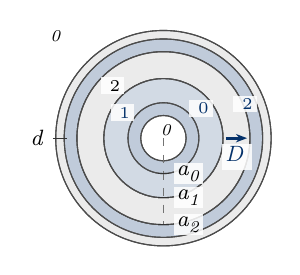
\begin{tikzpicture}[line join=round]
\filldraw[draw=black!70,fill=black!8] (2.196,-1.620) circle (1.368);
\filldraw[draw=black!70,fill=FAUblue!25] (2.196,-1.620) circle (1.260);
\filldraw[draw=black!70,fill=white] (2.196,-1.620) circle (1.098);
\filldraw[draw=black!70,fill=black!8] (2.196,-1.620) circle (1.098);
\filldraw[draw=black!70,fill=white] (2.196,-1.620) circle (0.756);
\filldraw[draw=black!70,fill=FAUblue!18] (2.196,-1.620) circle (0.756);
\filldraw[draw=black!70,fill=FAUblue!25] (2.196,-1.620) circle (0.450);
\filldraw[draw=black!70,fill=white] (2.196,-1.620) circle (0.288);
\draw[black!70] (2.196,-1.620) circle (1.368);
\draw[black!70] (2.196,-1.620) circle (1.260);
\draw[black!70] (2.196,-1.620) circle (1.098);
\draw[black!70] (2.196,-1.620) circle (0.756);
\draw[black!70] (2.196,-1.620) circle (0.450);
\draw[black!70] (2.196,-1.620) circle (0.288);
\draw[-{Stealth[length=4pt]},FAUblue,line width=1.2pt] (2.988,-1.620) -- (3.258,-1.620);
\node[,inner sep=1pt,font=\footnotesize] at (2.196,-1.512) {\textit{ε\textsubscript{0}}};
\node[text=FAUblue,fill=white,fill opacity=0.85,text opacity=1,inner sep=1pt,font=\footnotesize] at (1.674,-1.296) {ε\textsubscript{1}};
\node[fill=white,fill opacity=0.85,text opacity=1,inner sep=1pt,font=\footnotesize] at (1.548,-0.954) {ε\textsubscript{2}};
\node[,inner sep=1pt,font=\footnotesize] at (0.792,-0.324) {\textit{ε\textsubscript{0}}};
\node[anchor=west,text=FAUblue,fill=white,fill opacity=0.85,text opacity=1,inner sep=1pt,font=\footnotesize] at (2.520,-1.242) {σ\textsubscript{0}};
\node[anchor=west,text=FAUblue,fill=white,fill opacity=0.85,text opacity=1,inner sep=1pt,font=\footnotesize] at (3.078,-1.188) {σ\textsubscript{2}};
\node[text=FAUblue,fill=white,fill opacity=0.85,text opacity=1,inner sep=1pt,font=\footnotesize] at (3.132,-1.854) {\textit{D\textsubscript{ρ}}};
\draw[black!55,dashed] (2.196,-1.620) -- (2.196,-2.718);
\draw[black!80] (2.124,-2.070) -- (2.268,-2.070);
\node[anchor=west,fill=white,fill opacity=0.85,text opacity=1,inner sep=1pt,font=\footnotesize] at (2.322,-2.070) {\textit{a\textsubscript{0}}};
\draw[black!80] (2.124,-2.376) -- (2.268,-2.376);
\node[anchor=west,fill=white,fill opacity=0.85,text opacity=1,inner sep=1pt,font=\footnotesize] at (2.322,-2.376) {\textit{a\textsubscript{1}}};
\draw[black!80] (2.124,-2.718) -- (2.268,-2.718);
\node[anchor=west,fill=white,fill opacity=0.85,text opacity=1,inner sep=1pt,font=\footnotesize] at (2.322,-2.718) {\textit{a\textsubscript{2}}};
\draw[black!80] (0.792,-1.620) -- (0.972,-1.620);
\node[anchor=east,inner sep=1pt,font=\footnotesize] at (0.720,-1.620) {\textit{d}};
\end{tikzpicture}\par\smallskip{\small\raggedright \textbf{Track each cylindrical boundary by radius.} The field runs radially through ε\textsubscript{1} then ε\textsubscript{2}; free surface charges sit on the two metal faces bordering the dielectric gap.\par}\end{minipage}
\end{center}

In the dielectric gap, symmetry gives \textit{D} = \textit{D}\textsubscript{ρ}(ρ)\textit{e}\textsubscript{ρ}. The sheet fixes the voltage direction: \textit{U}\textsubscript{20} = $\int $ from P\textsubscript{2} (outer) to P\textsubscript{0} (inner) of \textit{E} \ensuremath{\cdot} d\textit{s}, matching the figure’s arrow from the outer to the inner terminal and the course convention \textit{U}\textsubscript{20} = φ\textsubscript{2} \ensuremath{-} φ\textsubscript{0}. The path therefore runs inward.

\begin{keepsection}
\Needspace{7\baselineskip}
\subsection{10a: Flux density, field, and outer surface charge}

\Needspace{4\baselineskip}
Try first: apply cylindrical Gauss surfaces in each dielectric, then use continuity of normal D at ρ = a\textsubscript{1} and the conductor boundary at ρ = a\textsubscript{2}.

\nopagebreak[4]{\small\itshape Answers: see “Task 10: Two-dielectric coaxial capacitor” under Answers at the end.}
\end{keepsection}

\begin{keepsection}
\Needspace{7\baselineskip}
\subsection{10b: Field and σ\textsubscript{0} as functions of U\textsubscript{20}}

\Needspace{4\baselineskip}
Try first: integrate E along the path the sheet gives, inward from P\textsubscript{2} at a\textsubscript{2} to P\textsubscript{0} at a\textsubscript{0}, splitting at a\textsubscript{1}, then solve the voltage relation for σ\textsubscript{0}.

\nopagebreak[4]{\small\itshape Answers: see “Task 10: Two-dielectric coaxial capacitor” under Answers at the end.}
\end{keepsection}

\begin{keepsection}
\Needspace{6\baselineskip}
\subsection{10c: Capacitance for length Δz}

\Needspace{3\baselineskip}
Try first: use the inner conductor’s charge over length Δz and divide by the voltage from 10b.

\nopagebreak[4]{\small\itshape Answers: see “Task 10: Two-dielectric coaxial capacitor” under Answers at the end.}
\end{keepsection}

\begin{keepsection}
\Needspace{7\baselineskip}
\subsection{10d: Field inside the inner conductor and outside the outer one}

\Needspace{4\baselineskip}
Try first: use Gauss’s law and the conductor condition D = 0, remembering that the two facing surface charges cancel per unit length.

\nopagebreak[4]{\small\itshape Answers: see “Task 10: Two-dielectric coaxial capacitor” under Answers at the end.}
\end{keepsection}
\end{keepsection}


\clearpage
\section{Answers}
\begin{keepsection}\subsection{Task 9: Field at a flat dielectric boundary}

\begin{workedbox}{9 \ensuremath{\cdot} Apply both interface conditions}
\Needspace{14\baselineskip}
\begin{enumerate}
\item \Needspace{5\baselineskip}
The interface is horizontal, so its normal is along y and its tangent is along x. There is no free charge sheet in the problem. Therefore:

\begin{equation*}{E}_{1\mathrm{x}}\, =\, {E}_{0\mathrm{x}};\, \quad \, {D}_{1\mathrm{y}}\, =\, {D}_{0\mathrm{y}},\, \quad \, \text{equivalently}\, {ε}_{1}{E}_{1\mathrm{y}}\, =\, {ε}_{0}{E}_{0\mathrm{y}}\end{equation*}
\item \Needspace{4\baselineskip}
First evaluate the given air field at y = h. Its tangential component is:

\begin{equation*}{E}_{0\mathrm{x}}(\mathrm{x},\mathrm{h})\, =\, \dfrac{{λ}_{0}\mathrm{x}}{π({ε}_{0}\, +\, {ε}_{1})(\mathrm{x}^{2}\, +\, \mathrm{h}^{2})}\end{equation*}
\item \Needspace{4\baselineskip}
Keep that x-component unchanged across the boundary:

\begin{equation*}{E}_{1\mathrm{x}}(\mathrm{x},\mathrm{h})\, =\, {E}_{0\mathrm{x}}(\mathrm{x},\mathrm{h})\end{equation*}
\item \Needspace{5\baselineskip}
The measured normal component contains the factor ε\textsubscript{1}/ε\textsubscript{0}. Multiplying it by ε\textsubscript{0}/ε\textsubscript{1} to preserve D cancels that factor:

\begin{equation*}{E}_{1\mathrm{y}}(\mathrm{x},\mathrm{h})\, =\, \dfrac{{ε}_{0}}{{ε}_{1}}{E}_{0\mathrm{y}}(\mathrm{x},\mathrm{h})\, =\, \dfrac{{λ}_{0}\mathrm{h}}{π({ε}_{0}\, +\, {ε}_{1})(\mathrm{x}^{2}\, +\, \mathrm{h}^{2})}\end{equation*}
\item \Needspace{4\baselineskip}
\textbf{Result:} combine the two components into the dielectric-side vector:

\Needspace{5\baselineskip}
\begin{equation*}{E}_{1}(\mathrm{x},\mathrm{h})\, =\, \dfrac{{λ}_{0}}{π({ε}_{0}\, +\, {ε}_{1})(\mathrm{x}^{2}\, +\, \mathrm{h}^{2})}\, [\mathrm{x}{e}_{\mathrm{x}}\, +\, \mathrm{h}{e}_{\mathrm{y}}]\end{equation*}

\textbf{Check:} the tangential component is unchanged; the normal flux density matches on both sides. With SI inputs, E is in V/m (equivalently N/C).
\end{enumerate}
\end{workedbox}

\end{keepsection}
\begin{keepsection}\subsection{Task 10: Two-dielectric coaxial capacitor}

\begin{workedbox}{10a \ensuremath{\cdot} Use enclosed charge per unit length}
\Needspace{15\baselineskip}
\begin{enumerate}
\item \Needspace{6\baselineskip}
Choose a coaxial Gaussian cylinder of radius ρ and length Δz, with a\textsubscript{0} \ensuremath{<} ρ \ensuremath{<} a\textsubscript{2}. Radial D is constant over its curved side; its end caps contribute no flux. The enclosed free charge is the inner surface charge on length Δz:

\begin{equation*}{D}_{ρ}(ρ)\, 2πρ\, Δ{z}\, =\, σ_{0}\, 2π{a}_{0}\, Δ{z}\end{equation*}
\item \Needspace{5\baselineskip}
Cancel the common factors. No free charge lies at the dielectric boundary ρ = a\textsubscript{1}, so normal D has the same value in both layers:

\begin{equation*}{D}(ρ)\, =\, \dfrac{σ_{0}{a}_{0}}{ρ}\, {e}_{ρ},\, \quad \, {a}_{0}\, <\, ρ\, <\, {a}_{2}\end{equation*}
\item \Needspace{4\baselineskip}
Use D = εE separately in each material:

\Needspace{4\baselineskip}
\begin{equation*}{E}(ρ)\, =\, \dfrac{σ_{0}{a}_{0}}{ε_{1}ρ}{e}_{ρ},\, \quad \, {a}_{0}\, <\, ρ\, <\, {a}_{1}\end{equation*}

\begin{equation*}{E}(ρ)\, =\, \dfrac{σ_{0}{a}_{0}}{ε_{2}ρ}{e}_{ρ},\, \quad \, {a}_{1}\, <\, ρ\, <\, {a}_{2}\end{equation*}
\item \Needspace{5\baselineskip}
At the inner face of the outer metal cylinder, the normal from the conductor into the gap points inward, \ensuremath{-}e\textsubscript{ρ}. Thus σ\textsubscript{2} = D \ensuremath{\cdot} (\ensuremath{-}e\textsubscript{ρ}) at ρ = a\textsubscript{2}:

\Needspace{5\baselineskip}
\begin{equation*}σ_{2}\, =\, -\dfrac{σ_{0}{a}_{0}}{{a}_{2}}\end{equation*}

\Needspace{5\baselineskip}
\textbf{Result:} D is radial and continuous through the dielectric interface; E changes magnitude inversely with permittivity. The two metal-face charges have opposite signs.

\textbf{Check:} σ\textsubscript{2} 2πa\textsubscript{2}Δz = \ensuremath{-}σ\textsubscript{0} 2πa\textsubscript{0}Δz, so the two facing surfaces carry equal and opposite charge.
\end{enumerate}
\end{workedbox}

\end{keepsection}
\begin{keepsection}\subsection{Task 10: Two-dielectric coaxial capacitor}

\begin{workedbox}{10b \ensuremath{\cdot} Integrate through both layers}
\Needspace{17\baselineskip}
\begin{enumerate}
\item \Needspace{5\baselineskip}
The path runs inward, from ρ = \textit{a}\textsubscript{2} to ρ = \textit{a}\textsubscript{0}. Along a radial path d\textit{s} = \textit{e}\textsubscript{ρ} dρ, and the limits carry the direction, so \textit{E} \ensuremath{\cdot} d\textit{s} = \textit{E}\textsubscript{ρ} dρ with ρ decreasing. Insert the two E expressions from 10a:

\begin{equation*}{U}_{20}\, =\, \int_{{a}_{2}}^{{a}_{1}} \, \dfrac{σ_{0}{a}_{0}}{ε_{2}ρ}\, \mathrm{d}ρ\, +\, \int_{{a}_{1}}^{{a}_{0}} \, \dfrac{σ_{0}{a}_{0}}{ε_{1}ρ}\, \mathrm{d}ρ\end{equation*}
\item \Needspace{5\baselineskip}
Each integral of 1/ρ gives a logarithm; running inward makes each one negative, for example $\int $ from \textit{a}\textsubscript{1} to \textit{a}\textsubscript{0} of dρ/ρ = ln(\textit{a}\textsubscript{0}/\textit{a}\textsubscript{1}) = \ensuremath{-}ln(\textit{a}\textsubscript{1}/\textit{a}\textsubscript{0}):

\begin{equation*}{U}_{20}\, =\, -σ_{0}{a}_{0}\left[\dfrac{1}{ε_{1}}\, \ln \dfrac{{a}_{1}}{{a}_{0}}\, +\, \dfrac{1}{ε_{2}}\, \ln \dfrac{{a}_{2}}{{a}_{1}}\right]\end{equation*}
\item \Needspace{4\baselineskip}
Define the positive geometry/material factor:

\begin{equation*}{S}\, =\, \dfrac{1}{ε_{1}}\, \ln \dfrac{{a}_{1}}{{a}_{0}}\, +\, \dfrac{1}{ε_{2}}\, \ln \dfrac{{a}_{2}}{{a}_{1}}\end{equation*}
\item \Needspace{4\baselineskip}
Rearrange for the inner surface charge density, then substitute it back into D and E:

\Needspace{4\baselineskip}
\begin{equation*}σ_{0}\, =\, -\dfrac{{U}_{20}}{{a}_{0}{S}};\, \quad \, {D}(ρ)\, =\, -\dfrac{{U}_{20}}{{S}ρ}{e}_{ρ}\end{equation*}

\Needspace{4\baselineskip}
\begin{equation*}{E}(ρ)\, =\, -\dfrac{{U}_{20}}{ε_{1}{S}ρ}{e}_{ρ},\, \quad \, {a}_{0}\, <\, ρ\, <\, {a}_{1}\end{equation*}

\begin{equation*}{E}(ρ)\, =\, -\dfrac{{U}_{20}}{ε_{2}{S}ρ}{e}_{ρ},\, \quad \, {a}_{1}\, <\, ρ\, <\, {a}_{2}\end{equation*}
\item \Needspace{8\baselineskip}
\textbf{Result:} for positive U\textsubscript{20} the outer cylinder is at the higher potential, so σ\textsubscript{0} \ensuremath{<} 0, σ\textsubscript{2} = \ensuremath{-}σ\textsubscript{0}\textit{a}\textsubscript{0}/\textit{a}\textsubscript{2} \ensuremath{>} 0, and the field points inward, from the outer cylinder to the inner one.

\textbf{Check:} the field points from high to low potential, and the outer cylinder (node 2) is high when U\textsubscript{20} \ensuremath{>} 0, so an inward field is right. Integrating the resulting E inward from \textit{a}\textsubscript{2} to \textit{a}\textsubscript{0} returns +U\textsubscript{20}. Likely mistake: integrating outward from P\textsubscript{0} to P\textsubscript{2}, which flips every sign. The field has units V/m and σ\textsubscript{0} has units C/m².
\end{enumerate}
\end{workedbox}

\end{keepsection}
\begin{keepsection}\subsection{Task 10: Two-dielectric coaxial capacitor}

\begin{workedbox}{10c \ensuremath{\cdot} Capacitance per unit length}
\Needspace{9\baselineskip}
\begin{enumerate}
\item \Needspace{5\baselineskip}
Capacitance is the charge on the electrode at the higher potential divided by the voltage. For U\textsubscript{20} \ensuremath{>} 0 that is the outer cylinder, whose facing surface carries Q = σ\textsubscript{2} 2π\textit{a}\textsubscript{2}Δ\textit{z} = \ensuremath{-}σ\textsubscript{0} 2π\textit{a}\textsubscript{0}Δ\textit{z}:

\begin{equation*}{C}\, =\, \dfrac{{Q}}{{U}_{20}}\, =\, \dfrac{-σ_{0}2π{a}_{0}Δ{z}}{{U}_{20}}\end{equation*}
\item \Needspace{4\baselineskip}
Substitute σ\textsubscript{0} = \ensuremath{-}U\textsubscript{20}/(a\textsubscript{0}S). The signs, the voltage and a\textsubscript{0} cancel:

\begin{equation*}{C}\, =\, \dfrac{2πΔ{z}}{{S}};\, \quad \, {C}_{\mathrm{B}}\, =\, \dfrac{{C}}{Δ{z}}\, =\, \dfrac{2π}{{S}}\end{equation*}
\item \Needspace{5\baselineskip}
\textbf{Result:} C is the capacitance over length Δz; C\textsubscript{B} is the capacitance loading per unit length.

\textbf{Check:} S has units m/F, so C is in farads and C\textsubscript{B} in F/m. If ε\textsubscript{1} = ε\textsubscript{2} = ε, then S = ln(a\textsubscript{2}/a\textsubscript{0})/ε, recovering the homogeneous coaxial result.
\end{enumerate}
\end{workedbox}

\end{keepsection}
\begin{keepsection}\subsection{Task 10: Two-dielectric coaxial capacitor}

\begin{workedbox}{10d \ensuremath{\cdot} Zero field outside the charged gap}
\Needspace{10\baselineskip}
\begin{enumerate}
\item For 0 \ensuremath{\leq} ρ \ensuremath{<} a\textsubscript{0}, a coaxial Gaussian cylinder encloses no free charge: σ\textsubscript{0} lies at ρ = a\textsubscript{0}, outside this Gaussian surface. Thus its radial flux and field are zero. Within the inner metal wall D is also zero by the conductor condition.
\item \Needspace{5\baselineskip}
For ρ \ensuremath{>} a\textsubscript{2}, a Gaussian cylinder outside both facing surfaces encloses their total charge per length:

\Needspace{5\baselineskip}
\begin{equation*}\dfrac{{q}_{\text{enc}}}{Δ{z}}\, =\, 2π{a}_{0}σ_{0}\, +\, 2π{a}_{2}σ_{2}\, =\, 0\end{equation*}

The cancellation uses σ\textsubscript{2} = \ensuremath{-}σ\textsubscript{0}a\textsubscript{0}/a\textsubscript{2}. Therefore D and E vanish outside the outer conductor; they also vanish within its metal wall.
\item \Needspace{4\baselineskip}
\textbf{Result:}

\Needspace{4\baselineskip}
\begin{equation*}{E}\, =\, 0,\, \quad \, 0\, \leq \, ρ\, <\, {a}_{0}\end{equation*}

\Needspace{5\baselineskip}
\begin{equation*}{E}\, =\, 0,\, \quad \, ρ\, >\, {a}_{2}\end{equation*}

\textbf{Check:} the applied voltage and field are confined to the annular dielectric gap in this ideal infinitely long, concentric arrangement.
\end{enumerate}
\end{workedbox}

\end{keepsection}

\vfill{\small Personal worked-solution guide based on the supplied EEI Exercise 4 sheet, written in my own words; no exercise text or figures are reproduced. Not an official FAU publication; check course details against current material. Made by \textbf{Thanate Amornjiraporn (Focus)}.}

\end{document}
